A \ac{CNN} is a special kind of neural network, and it was one of the first deep learning models to perform well in commercial applications. A \ac{CNN} is loosely based on principles drawn from neuroscience. According to \cite{Bengio_deep_learning_book},  local connectivity and parameter sharing are properties characteristic for \ac{CNN}s. These properties and the architecture of \ac{CNN}s will be explored further below.

\subsubsection{Convolution}
In mathematics, convolution is a mathematical operation on two real-valued functions that express the amount of overlap of one function as it is shifted over another function. For machine learning applications, the data is usually discretized. The operation is therefore a discrete summation over the data, and is used to calculate the weighted sum between the activations and the connection weights in a \ac{CNN}. The discrete convolution operation without kernel-flipping:

$$ (x*w)(t) = \sum\limits_{a=-\infty}^\infty x[a]w[t+a]$$ 

For aerial images we extend the convolution operation to two dimensions, and limit the summation to a finite number of pixels. To convolve an image I, a two-dimensional kernel K containing the weights is shifted across the image:  

$$ (I*K)[i,j] = \sum\limits_{m}\sum\limits_{n} I[i+m, j+n]K[m,n]$$ 

This operation is  visualized in figure \ref{fig:convolution} where a $2 \times 2$ kernel of weights is convolved with a $3 \times 3$ matrix of input values, and produces $2 \times 3$ outputs. 

\begin{figure}[t]
\begin{center}
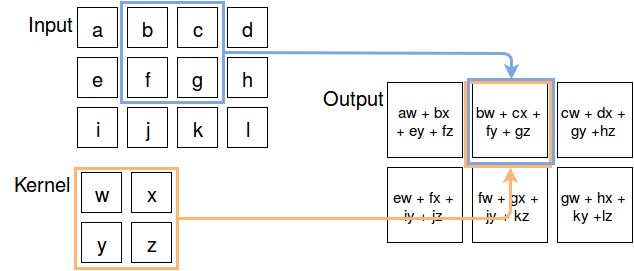
\includegraphics[width=0.8\columnwidth]{figs/convolution.png}
\caption[Convolution example]{Example of 2D convolution without kernel-flipping.}
\label{fig:convolution}
\end{center}
\end{figure}


\subsubsection{Local Connectivity}
In a traditional neural network each layer is typically fully connected. Each unit has connections to every unit in the previous layer. In a \ac{CNN}, however, a unit  interacts only with a small region of units in the previous layer. This region is often referred to as the unit's local receptive field. This kind of local connectivity can be very practical for high-dimensional data, such as images where meaningful features can be extracted using only a small area of the total image. \\

Local connectivity can be achieved by using a small kernel as seen in Figure \ref{fig:convolution}. Instead of each output unit being connected to all inputs, the output only depends on a $2 \times 2$ region for summation. \\

If there are $m$ inputs and $n$ output units, a matrix multiplication for a fully-connected network would require $m\times n$ parameters, as well as having a runtime of $O(m\times n)$. By using a kernel we limit the number of connections each output may have to k. This requires only $k\times n$ parameters and a runtime of $O(k\times n)$. For image applications the kernel size can be relatively small and still achieve good results, which can give big improvements in efficiency.

\subsubsection{Parameter Sharing}
The number of model parameters are further reduced by using parameter sharing. Each weight in the kernel is applied to every position of the input. In contrast, a neural network which is fully connected will have a separate weight for every connection. This can be redundant for high-dimensional data, where most of the features are localized. In images, for example, an important feature to extract are edges. A kernel with weights that are good at detecting edges at one location, will be equally good at detecting them in other locations. \\

The use of parameter sharing further reduces the storage requirement to $k$ parameters. Usually one kernel per layer is not enough, so several kernels with tied weights convolve the input. The layer will then produce output activations for different features. The output of several kernels are often referred to as feature maps.

\subsubsection{Pooling}
The pooling function is another operation typically associated with \ac{CNN}. A pooling function modifies the output of a layer in some way. It replaces a rectangular region of the output by a single value that has been determined by a summary operation. A common pooling function is the max pooling operation, which outputs the maximum within a rectangular neighbourhood. The reason for utilizing pooling is that it helps the representation become invariant to small translation in the input. For example a network created to classify whether an image depicts a cat or not will benefit from pooling, since the location of the cat in the picture is irrelevant. For tasks where the location of a feature is important, such as semantic segmentation, applying pooling should be done with restraint. Additionally, pooling reduce the number of input parameters for the next layer.

\subsubsection{Layer Structure}
A typical convolutional layer in a network consists of three stages. First, convolution sums the weighted inputs \todo{Correct to say?}. Second, an activation function is applied to the summed, weighted inputs \todo{Sounds weird} for all units in the layer. The rectified linear unit is a popular choice, and outputs either 0 or the weighted sum \todo{Here as well}, depending on which is biggest. $f(x) = max(0, a)$. Finally the pooling function modifies the output of the layer. 

\subsubsection{Network architecture}
A \ac{CNN} usually consists of both convolutional layers and fully-connected layers. The input layer and the initial hidden layers are convolutional layers, with fully connected layers attached at the end. Figure \ref{fig:conv} shows a convolutional neural network configuration. The input layer and the two first hidden layers are convolutional layers. During training, the kernel weights for these layers are adjusted by back-propagation. Each feature map defines a set of kernel weights that are applied to all input pixels or activations. Usually, a \ac{CNN} will reduce the necessity of feature engineering because it learns what suitable features to extract from input data. In images, a \ac{CNN} is able to learn from raw pixel values without the use of feature extraction techniques found in computer vision.


\begin{figure}[t]
\begin{center}
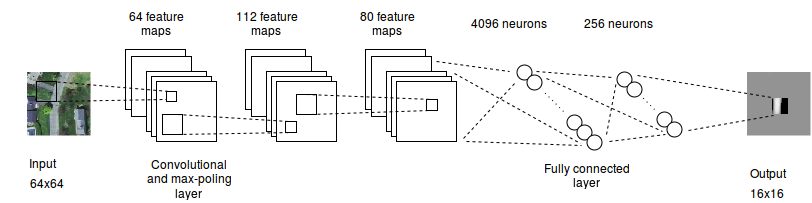
\includegraphics[width=1\columnwidth]{figs/conv_diagram.png}
\caption[Convolutional neural network]{Convolutional neural network. }
\label{fig:conv}
\end{center}
\end{figure}